
\begin{center}
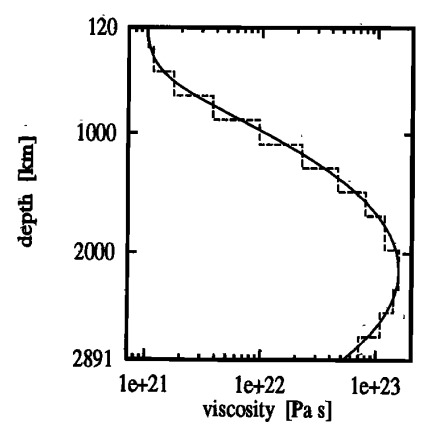
\includegraphics[width=6cm]{images/viscosity_profile/hamy95}\\
{\captionfont \nineteenninetyfive: Taken from Hanyk et al (1995) \cite{hamy95}. 
$\eta(z)=(1+214.3z\exp-16.7(0.7-z)^2)\times 10^{21}\si{pascal\second}$ }
\end{center}

\begin{center}
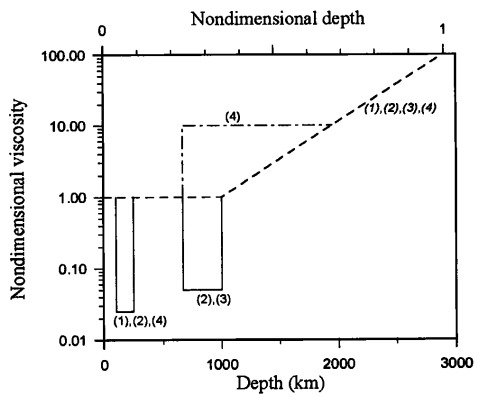
\includegraphics[width=6cm]{images/viscosity_profile/csyu97}\\
{\captionfont \nineteenninetyseven: Taken from Cserepes \& Yuen (1997) \cite{csyu97}} 
\end{center}

\begin{center}
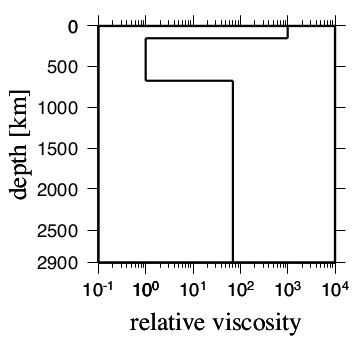
\includegraphics[width=5cm]{images/viscosity_profile/yohk01}\\
{\captionfont \twothousandone:Radial viscosity profile of the reference model. 3-layered model is adopted: 
the lithosphere (0 km to 150 km), the upper mantle (150 km to 670km) 
and the lower mantle (670 km to 2900 km). Taken from \cite{yohk01}}
\end{center}


\begin{center}
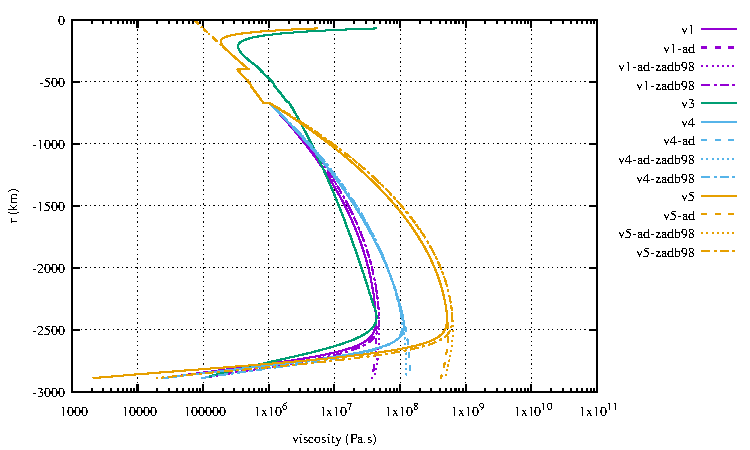
\includegraphics[height=6cm]{images/viscosity_profile/profiles_steinberger}
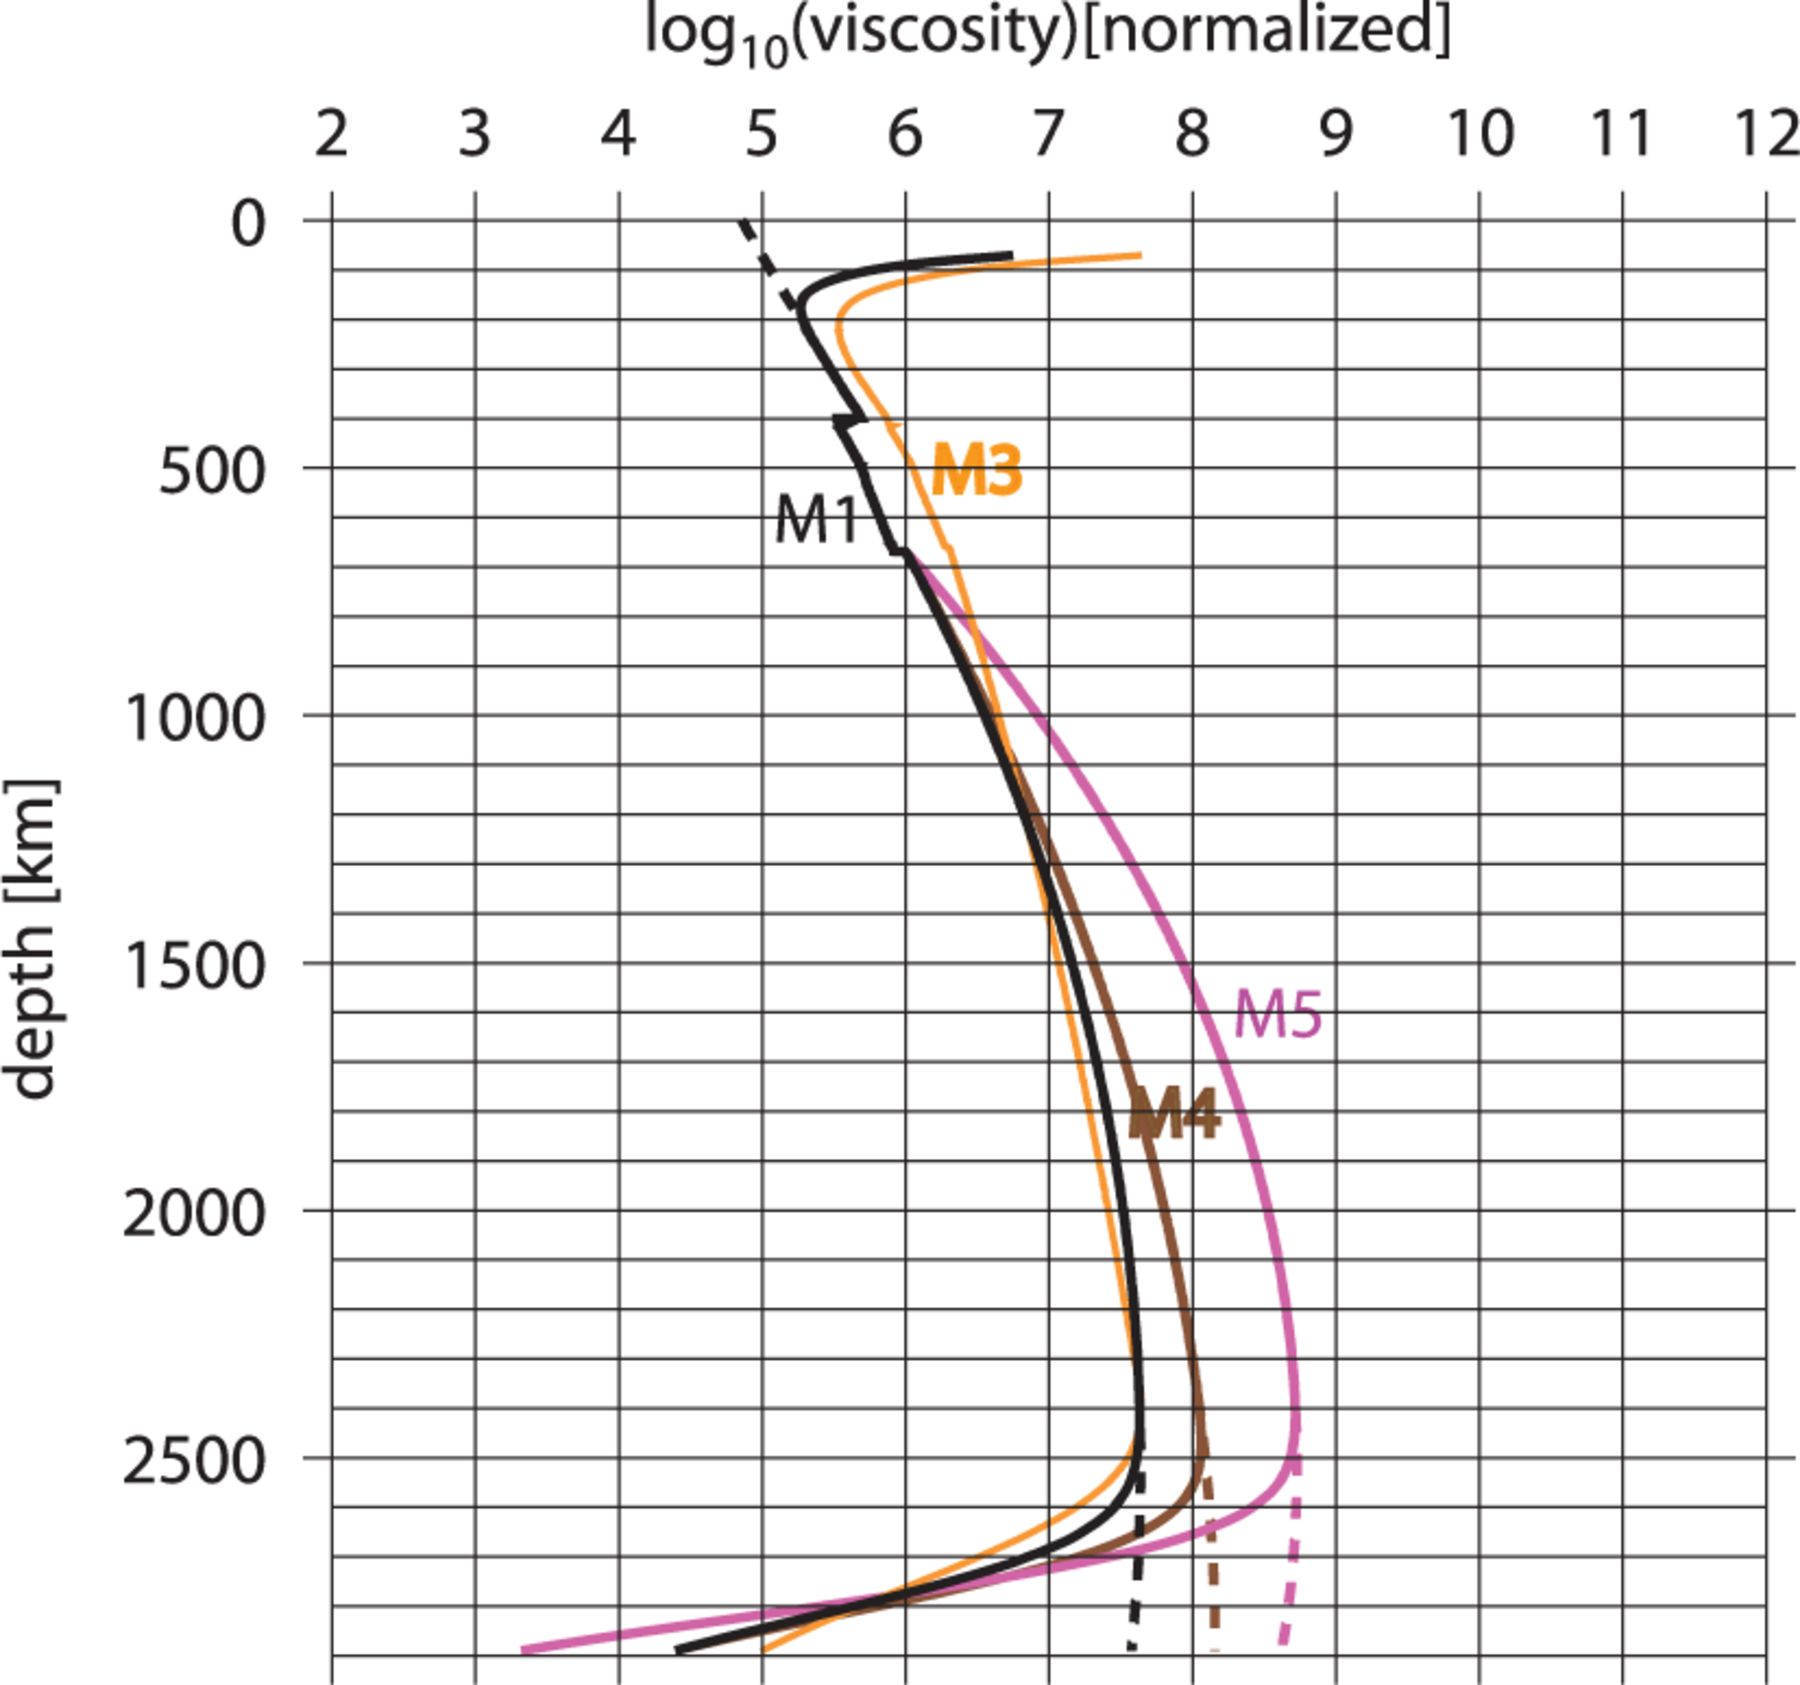
\includegraphics[height=6cm]{images/viscosity_profile/stca06-fig4}\\
{\captionfont \twothousandsix:
Non-optimized, normalized viscosity profiles, as sent by B. Steinberger,
corresponding to fig.~4 in Steinberger \& Calderwood (2006) \cite{stca06}.}
\end{center}


\begin{center}
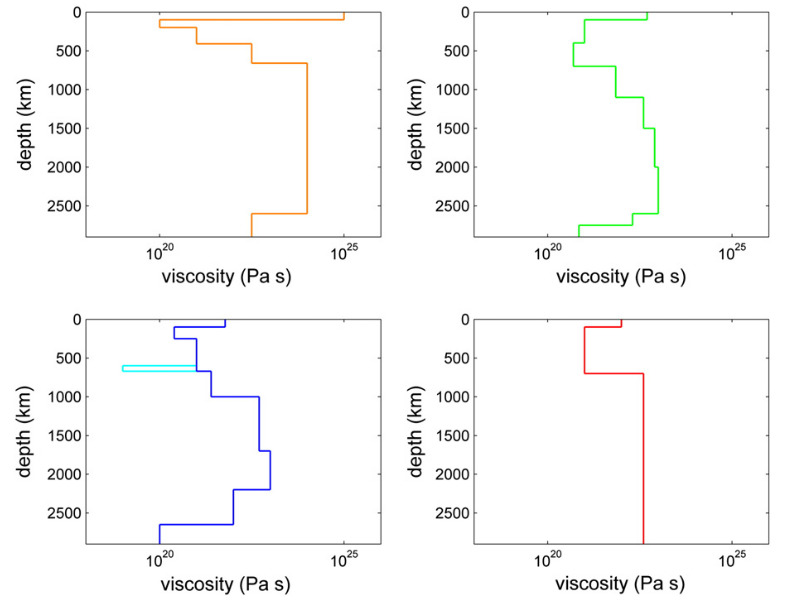
\includegraphics[width=11cm]{images/viscosity_profile/capd11}\\
{\captionfont \twothousandeleven: Taken from Cadio et al \cite{capd11}.
Mantle viscosity structure employed in calculating synthetic geoid anomalies. 
Red: VR (Ricard et al., 1993); Blue: VMF (Mitrovica and Forte, 2004); Cyan: VMF-LVZ (Mitrovica
and Forte, 2004); Green: VSC (Steinberger and Calderwood, 2006); Orange: VYN (Yoshida and Nakakuki, 2009).}
\end{center}

\begin{center}
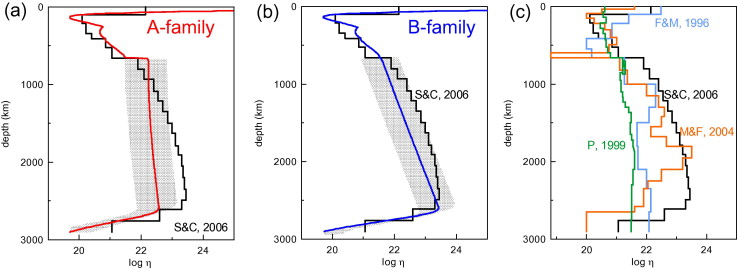
\includegraphics[width=11cm]{images/viscosity_profile/civs12-fig1}\\
{\captionfont \twothousandtwelve: Taken from Ciskova et al \cite{civs12}.}
\end{center}

\begin{center}
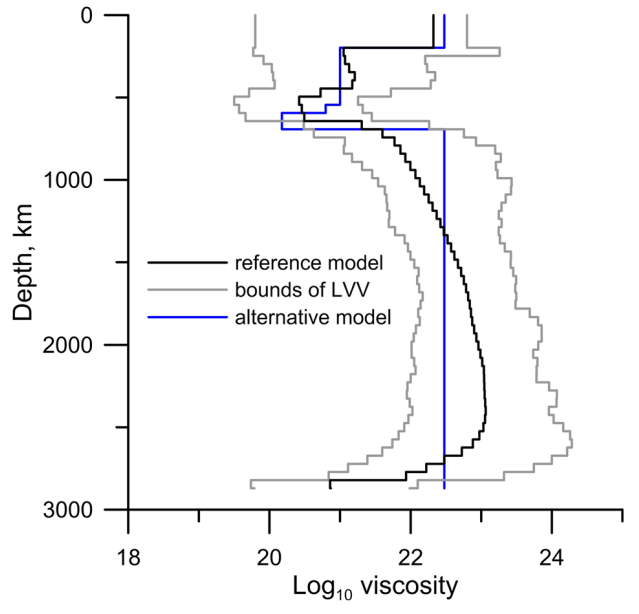
\includegraphics[width=6cm]{images/viscosity_profile/kaps14}\\
{\captionfont \twothousandfourteen Taken from Kaban \etal  \cite{kaps14}.
(Black) reference radial viscosity from (Steinberger and Calderwood 2006); 
(Blue) alternative viscosity model of Kaban and Trubitsyn (2012); 
(Light Grey) limits of viscosity variations in the model with LVV (Petrunin et al. 2013).
}
\end{center}


---------------------------------------------------------------------------

\begin{center}
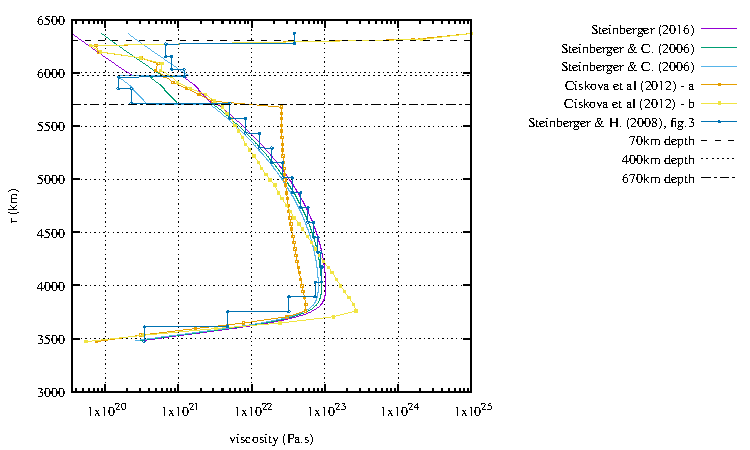
\includegraphics[width=14cm]{images/viscosity_profile/profiles}\\
{\captionfont Steinberger (2016) \cite{stei16}; 
Ciskova et al (2012) \cite{civs12}.}
\end{center}


\Literature:
\begin{itemize} 
\item Viscosity profile of the lower mantle \cite{elss85}
\item Matyska et al (2011) \cite{mayw11}
\item Flament (2019) \cite{flam19}
\item Mitrovica \& Forte \cite{mifo04}
\item King \& Masters \cite{kima92}
\item Rudolph et al \cite{rull15}
\item steinberger \& holme \cite{stho08}
\item steinberger \cite{stei16}
\item Cadek \& Yuen \cite{cayu93}
\item supp of \cite{badw17}
\end{itemize} 
